% !TEX root = ../slides_ISSTA.tex
%\subsection{Feature Analysis}
%{
%%\setbeamertemplate{background canvas}{\tikz[remember picture]\node[opacity=0.5] at (current page.center) {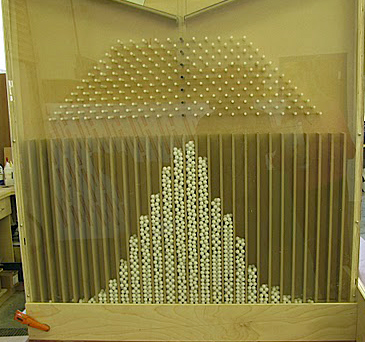
\includegraphics[keepaspectratio]{../nontex/illustrations/galtonBoard.jpg}};}
%\begin{frame}
%\frametitle{What Features Are Used Most Frequently?}
%\begin{block}{\begin{Large}Regex Feature Usage References Are Missing\end{Large}}
%\begin{itemize}
%\item \begin{large}feature usage statistics\end{large}
%\item \begin{large}feature set summaries for variants and tools\end{large}
%\end{itemize}
%\end{block}
%\end{frame}
%}
%\note[itemize]{
%    \item the first usage study...
%    \item put yourself in the shoes of a tool designer...
%    \item there is no reference...
%    \item basic idea is to get a bunch of regexes, and count how often their features are used
%}

\subsection{Sampling}

\begin{frame}
\frametitle{Part 2: Features}

\begin{block}{RQ3}
Which regular expression language features are most commonly used in Python?
\end{block}
\end{frame}

\begin{frame}
\frametitle{Project selection with the GitHub API}
\begin{columns}[t]
\column{.5\textwidth} % Left column and width
\begin{figure}[ht]
  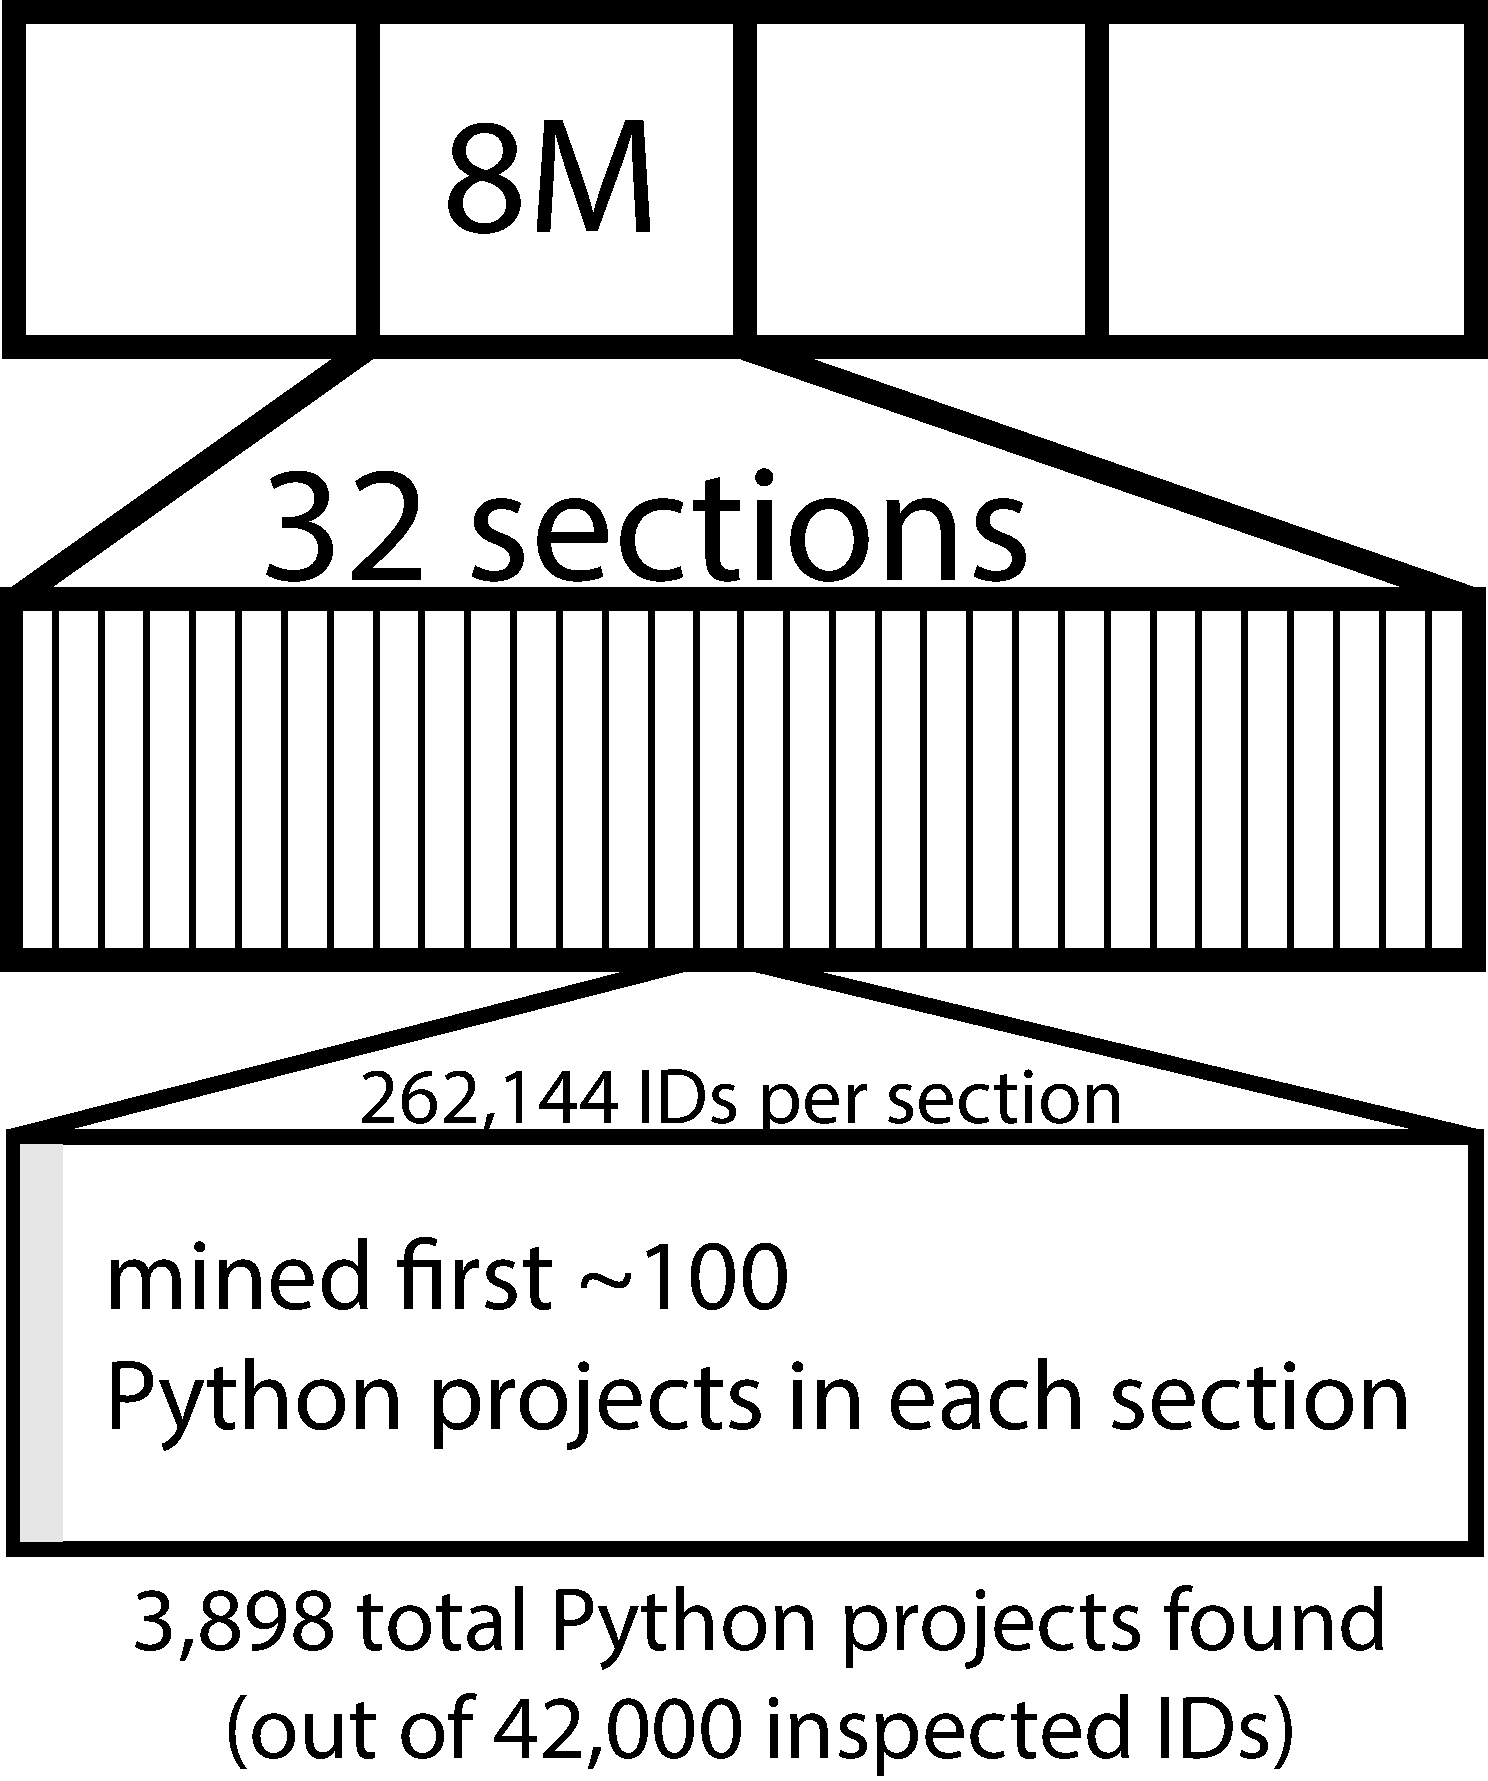
\includegraphics[scale=0.16]{../nontex/illustrations/32Divided.pdf}
  \label{fig:32Divided}
\end{figure}
\column{.5\textwidth} % Right column and width
\begin{figure}[ht]
  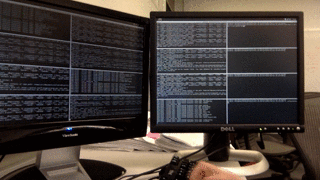
\includegraphics[width=\linewidth]{../nontex/smallScrapersPNG/smallScrapers-112}
  % \animategraphics[loop,width=\linewidth]{10}{nontex/smallScrapersPNG/smallScrapers-}{0}{400}
    \label{fig:scraper}
\end{figure}
Of 3,898 Python projects, 1,645 (42\%) called the {\tt re} module
\end{columns}
\end{frame}
\note[itemize]{
    \item in each section, average 1312 examined
    \item in each section, average 122 .py found
}

\begin{frame}
\frametitle{In Python: Utilizations of the re module}
\begin{figure}[h]
  \centering
  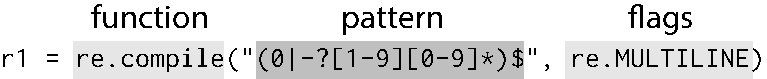
\includegraphics[scale=0.77]{../nontex/illustrations/exampleUsageLarge.pdf}
  \label{fig:exampleUsageLarge}
\end{figure}
\begin{description}
\item [function] which function of the re module is called?
\item [pattern] string used to specify regex behavior
\item [flags] modifies the regex engine
\end{description}
\end{frame}
\note[itemize]{
    \item 53,894 unique utilizations observed.
    \item pt 2
}


%------------------------------------------------




%------------------------------------------------

{
\setbeamertemplate{background canvas}{\tikz[remember picture,overlay]\node[opacity=0.3] at (current page.center) {
\includegraphics[width=\paperwidth,height=\paperheight,keepaspectratio]{nontex/illustrations/funnel.png}};}
\begin{frame}
\frametitle{Filtering utilizations and patterns}
\begin{itemize}
\item [] \textbf{53,894} unique utilizations observed in 1,645 projects.
\item [] \begin{footnotesize}12.7\% use behavioral flags\end{footnotesize}
\item [] \begin{footnotesize}6.5\% were non-static patterns\end{footnotesize}
\item [] \textbf{43,525} utilizations remain
\item<2-> [] \textbf{13,711} distinct  patterns
\item<2-> [] \begin{footnotesize}114 had various errors\end{footnotesize}
%\item [] \begin{footnotesize}17 had non-Python features\end{footnotesize}
%\item [] \begin{footnotesize}22 had various errors\end{footnotesize}
%\item [] \begin{footnotesize}2 had ECOM feature - too rare to include\end{footnotesize}
\item<3-> [] \textbf{13,597} patterns from 1,544 projects remain for analysis
\end{itemize}

%\onslide<4->
%\begin{block}{}
%Average utilizations per project: 32
%\end{block}

\end{frame}
}
\note[itemize]{
    \item pt 2
}

%------------------------------------------------

%
%\begin{frame}
%\frametitle{Utilization statistics}
%\begin{itemize}
%     \item average utilizations per project was 32 and the maximum was 1,427
%     \item each project had an average of 11 files containing any utilization, but med was 6, so there is a skew bc of a few projects with so many
%     \item each of these files had an average of 2 utilizations (med 1)
%     \item avg 2 util. per file
%     \item max 207 util. per file
%     \item max 541 files w/utilizations, med was 2, Q3 was 6...this got skewed
%\end{itemize}
%\end{frame}



 \begin{frame}
 \frametitle{PCRE parsing patterns}
 \begin{figure}[h]
   \centering
   \includegraphics[scale=1.25]{nontex/illustrations/featureParsing.pdf}
   \label{fig:featureParsing}
 \end{figure}
 \begin{center}
 \begin{Large}
% \onslide<2->
% All Python features are recognizable by PCRE
 \end{Large}
 \end{center}
 \end{frame}
 \note[itemize]{
     \item pt 1
     \item pt 2
 }

% %------------------------------------------------

%\begin{frame}[fragile]
%\frametitle{Feature Statistics}
%\begin{columns}[t]
\column{.47\textwidth}
\begin{adjustbox}{totalheight=\textheight-9\baselineskip}
\begin{tabular}
{lllcccc  cc}
\textbf{Rank} & \textbf{Code} & \textbf{Example} & \% \textbf{Projects} & \textbf{NProjects} & \textbf{NFiles} & \textbf{NPatterns} & \textbf{MaxTokens} \\
\toprule[0.12em]
1 & ADD & \begin{minipage}{0.5in}\begin{verbatim}z+\end{verbatim}\end{minipage} & 73.2 & 1,204 & 9,165 & 6,003 & 30 \\
\midrule
2 & CG & \begin{minipage}{0.5in}\begin{verbatim}(caught)\end{verbatim}\end{minipage} & 72.6 & 1,194 & 9,559 & 7,130 & 17 \\
\midrule
3 & KLE & \begin{minipage}{0.5in}\begin{verbatim}.*\end{verbatim}\end{minipage} & 66.8 & 1,099 & 8,163 & 6,017 & 50 \\
\midrule
4 & CCC & \begin{minipage}{0.5in}\begin{verbatim}[aeiou]\end{verbatim}\end{minipage} & 62.4 & 1,026 & 7,648 & 4,468 & 42 \\
\midrule
5 & ANY & \begin{minipage}{0.5in}\begin{verbatim}.\end{verbatim}\end{minipage} & 61.1 & 1,005 & 6,277 & 4,657 & 60 \\
\midrule
6 & RNG & \begin{minipage}{0.5in}\begin{verbatim}[a-z]\end{verbatim}\end{minipage} & 51.6 & 848 & 5,092 & 2,631 & 50 \\
\midrule
7 & STR & \begin{minipage}{0.5in}\begin{verbatim}^\end{verbatim}\end{minipage} & 51.4 & 846 & 5,458 & 3,563 & 12 \\
\midrule
8 & END & \begin{minipage}{0.5in}\begin{verbatim}$\end{verbatim}\end{minipage} & 50.3 & 827 & 5,393 & 3,169 & 12 \\
\midrule[0.10em]
9 & NCCC & \begin{minipage}{0.5in}\begin{verbatim}[^qwxf]\end{verbatim}\end{minipage} & 47.2 & 776 & 3,947 & 1,935 & 15 \\
\midrule
10 & WSP & \begin{minipage}{0.5in}\begin{verbatim}\s\end{verbatim}\end{minipage} & 46.3 & 762 & 4,704 & 2,846 & 32 \\
\midrule
11 & OR & \begin{minipage}{0.5in}\begin{verbatim}a|b\end{verbatim}\end{minipage} & 43 & 708 & 3,926 & 2,102 & 15 \\
\midrule
12 & DEC & \begin{minipage}{0.5in}\begin{verbatim}\d\end{verbatim}\end{minipage} & 42.1 & 692 & 4,198 & 2,297 & 24 \\
\midrule
13 & WRD & \begin{minipage}{0.5in}\begin{verbatim}\w\end{verbatim}\end{minipage} & 39.5 & 650 & 2,952 & 1,430 & 13 \\
\midrule
14 & QST & \begin{minipage}{0.5in}\begin{verbatim}z?\end{verbatim}\end{minipage} & 39.2 & 645 & 3,707 & 1,871 & 35 \\
\midrule
15 & LZY & \begin{minipage}{0.5in}\begin{verbatim}z+?\end{verbatim}\end{minipage} & 36.8 & 605 & 2,221 & 1,300 & 12 \\
\midrule
16 & NCG & \begin{minipage}{0.5in}\begin{verbatim}a(?:b)c\end{verbatim}\end{minipage} & 24.6 & 404 & 1,709 & 791 & 28 \\
\midrule
17 & PNG & \begin{minipage}{0.5in}\begin{verbatim}(?P<name>x)\end{verbatim}\end{minipage} & 21.5 & 354 & 1,475 & 915 & 16 \\
\bottomrule[0.13em]
\end{tabular}
\end{adjustbox}
\column{.47\textwidth}
\begin{adjustbox}{totalheight=\textheight-9\baselineskip}
\begin{tabular}
{lllcccc  cc}
\textbf{Rank} & \textbf{Code} & \textbf{Example} & \% \textbf{Projects} & \textbf{NProjects} & \textbf{NFiles} & \textbf{NPatterns} & \textbf{MaxTokens} \\
\toprule[0.12em]
18 & SNG & \begin{minipage}{0.5in}\begin{verbatim}z{8}\end{verbatim}\end{minipage} & 20.7 & 340 & 1,267 & 581 & 17 \\
\midrule
19 & NWSP & \begin{minipage}{0.5in}\begin{verbatim}\S\end{verbatim}\end{minipage} & 16.4 & 270 & 776 & 484 & 10 \\
\midrule
20 & DBB & \begin{minipage}{0.5in}\begin{verbatim}z{3,8}\end{verbatim}\end{minipage} & 14.5 & 238 & 647 & 367 & 11 \\
\midrule
21 & NLKA & \begin{minipage}{0.5in}\begin{verbatim}a(?!yz)\end{verbatim}\end{minipage} & 11.1 & 183 & 489 & 131 & 3 \\
\midrule
22 & WNW & \begin{minipage}{0.5in}\begin{verbatim}\b\end{verbatim}\end{minipage} & 10.1 & 166 & 438 & 248 & 36 \\
\midrule
23 & NWRD & \begin{minipage}{0.5in}\begin{verbatim}\W\end{verbatim}\end{minipage} & 10 & 165 & 305 & 94 & 6 \\
\midrule
24 & LWB & \begin{minipage}{0.5in}\begin{verbatim}z{15,}\end{verbatim}\end{minipage} & 9.6 & 158 & 281 & 91 & 3 \\
\midrule
25 & LKA & \begin{minipage}{0.5in}\begin{verbatim}a(?=bc)\end{verbatim}\end{minipage} & 9.6 & 158 & 358 & 112 & 4 \\
\midrule
26 & OPT & \begin{minipage}{0.5in}\begin{verbatim}(?i)CasE\end{verbatim}\end{minipage} & 9.4 & 154 & 377 & 231 & 2 \\
\midrule
27 & NLKB & \begin{minipage}{0.5in}\begin{verbatim}(?<!x)yz\end{verbatim}\end{minipage} & 8.3 & 137 & 296 & 94 & 4 \\
\midrule
28 & LKB & \begin{minipage}{0.5in}\begin{verbatim}(?<=a)bc\end{verbatim}\end{minipage} & 7.3 & 120 & 255 & 80 & 4 \\
\midrule
29 & ENDZ & \begin{minipage}{0.5in}\begin{verbatim}\Z\end{verbatim}\end{minipage} & 5.5 & 90 & 149 & 89 & 1 \\
\midrule
30 & BKR & \begin{minipage}{0.5in}\begin{verbatim}\1\end{verbatim}\end{minipage} & 5.1 & 84 & 129 & 60 & 4 \\
\midrule
31 & NDEC & \begin{minipage}{0.5in}\begin{verbatim}\D\end{verbatim}\end{minipage} & 3.5 & 58 & 92 & 36 & 6 \\
\midrule
32 & BKRN & \begin{minipage}{0.5in}\begin{verbatim}(P?=name)\end{verbatim}\end{minipage} & 1.7 & 28 & 44 & 17 & 2 \\
\midrule
33 & VWSP & \begin{minipage}{0.5in}\begin{verbatim}\v\end{verbatim}\end{minipage} & 0.9 & 15 & 16 & 13 & 2 \\
\midrule
34 & NWNW & \begin{minipage}{0.5in}\begin{verbatim}\B\end{verbatim}\end{minipage} & 0.7 & 11 & 11 & 4 & 2 \\
\bottomrule[0.13em]
\end{tabular}
\end{adjustbox}
\end{columns}

%\end{frame}
%\note[itemize]{
%    \item pt 1
%    \item pt 2
%}

%\begin{frame}
%\frametitle{Feature analysis}
%  \centering
%  PCRE parser
%  
%  \includegraphics[scale=1.25]{../nontex/illustrations/featureParsing.pdf}
%
%\end{frame}

%------------------------------------------------


\begin{frame}[fragile]
\frametitle{Feature statistics - Top 8}
\begin{center}
\begin{adjustbox}{width=\textwidth}
\begin{tabular}
{lllcccc  cc}
\textbf{Rank} & \textbf{Code} & \textbf{Example} & \% \textbf{Projects} & \textbf{NProjects} & \textbf{NFiles} & \textbf{NPatterns} & \textbf{MaxTokens} \\
\toprule[0.12em]
1 & ADD & \begin{minipage}{0.5in}\begin{verbatim}z+\end{verbatim}\end{minipage} & 73.2 & 1,204 & 9,165 & 6,003 & 30 \\
\midrule
2 & CG & \begin{minipage}{0.5in}\begin{verbatim}(caught)\end{verbatim}\end{minipage} & 72.6 & 1,194 & 9,559 & 7,130 & 17 \\
\midrule
3 & KLE & \begin{minipage}{0.5in}\begin{verbatim}.*\end{verbatim}\end{minipage} & 66.8 & 1,099 & 8,163 & 6,017 & 50 \\
\midrule
4 & CCC & \begin{minipage}{0.5in}\begin{verbatim}[aeiou]\end{verbatim}\end{minipage} & 62.4 & 1,026 & 7,648 & 4,468 & 42 \\
\midrule
5 & ANY & \begin{minipage}{0.5in}\begin{verbatim}.\end{verbatim}\end{minipage} & 61.1 & 1,005 & 6,277 & 4,657 & 60 \\
\midrule
6 & RNG & \begin{minipage}{0.5in}\begin{verbatim}[a-z]\end{verbatim}\end{minipage} & 51.6 & 848 & 5,092 & 2,631 & 50 \\
\midrule
7 & STR & \begin{minipage}{0.5in}\begin{verbatim}^\end{verbatim}\end{minipage} & 51.4 & 846 & 5,458 & 3,563 & 12 \\
\midrule
8 & END & \begin{minipage}{0.5in}\begin{verbatim}$\end{verbatim}\end{minipage} & 50.3 & 827 & 5,393 & 3,169 & 12 \\
\bottomrule[0.13em]
\end{tabular}
\end{adjustbox}

\end{center}
\end{frame}
\note[itemize]{
    \item present in more than 50\% of projects
    \item pt 2
}



\begin{frame}
\frametitle{Regex research tools}

\begin{itemize}
\item Remember that we wanted to write a tool to support regex creation?
\item<2-> Regex feature usage references were missing (not anymore!).
\item <3-> So, 
\end{itemize}

\onslide<3->
\begin{block}{}%{\begin{Large}Regex Feature Usage References Are Missing\end{Large}}
\begin{large}We analyzed \emph{your} tools! (Hampi, Rex, RE2, brics, Automata.Z3)\end{large}
%\begin{itemize}
%\item \begin{large}feature usage statistics\end{large}
%\item \begin{large}feature set summaries for variants and tools\end{large}
%\end{itemize}
\end{block}


\end{frame}


%------------------------------------------------



%\begin{frame}[fragile]
%\frametitle{What Features Are Missing In Other Languages?}
%\begin{columns}[t]
\column{.47\textwidth}
\begin{adjustbox}{totalheight=\textheight-9\baselineskip}
\begin{tabular}{l@{  }clc@{  }lc @{   } c @{   }c @{   }c @{   }c @{   }c @{   }c @{   }c}\textbf{Rank} & \textbf{Code} & \textbf{Example} & \textbf{Python} & \textbf{Perl} & \textbf{.Net}  & \textbf{Ruby} &  \textbf{Java} & \textbf{RE2} & \textbf{JavaScript} & \textbf{POSIX ERE}\\
\toprule
1 & ADD & \begin{minipage}{0.5in}\begin{verbatim}z+\end{verbatim}\end{minipage} & \yes & \yes & \yes & \yes & \yes & \yes & \yes & \yes\\
\midrule
2 & CG & \begin{minipage}{0.5in}\begin{verbatim}(caught)\end{verbatim}\end{minipage} & \yes & \yes & \yes & \yes & \yes & \yes & \yes & \yes\\
\midrule
3 & KLE & \begin{minipage}{0.5in}\begin{verbatim}.*\end{verbatim}\end{minipage} & \yes & \yes & \yes & \yes & \yes & \yes & \yes & \yes\\
\midrule
4 & CCC & \begin{minipage}{0.5in}\begin{verbatim}[aeiou]\end{verbatim}\end{minipage} & \yes & \yes & \yes & \yes & \yes & \yes & \yes & \yes\\
\midrule
5 & ANY & \begin{minipage}{0.5in}\begin{verbatim}.\end{verbatim}\end{minipage} & \yes & \yes & \yes & \yes & \yes & \yes & \yes & \yes\\
\midrule
6 & RNG & \begin{minipage}{0.5in}\begin{verbatim}[a-z]\end{verbatim}\end{minipage} & \yes & \yes & \yes & \yes & \yes & \yes & \yes & \yes\\
\midrule
7 & STR & \begin{minipage}{0.5in}\begin{verbatim}^\end{verbatim}\end{minipage} & \yes & \yes & \yes & \yes & \yes & \yes & \yes & \yes\\
\midrule
8 & END & \begin{minipage}{0.5in}\begin{verbatim}$\end{verbatim}\end{minipage} & \yes & \yes & \yes & \yes & \yes & \yes & \yes & \yes\\
\midrule[0.10em]
9 & NCCC & \begin{minipage}{0.5in}\begin{verbatim}[^qwxf]\end{verbatim}\end{minipage} & \yes & \yes & \yes & \yes & \yes & \yes & \yes & \yes\\
\midrule
10 & WSP & \begin{minipage}{0.5in}\begin{verbatim}\s\end{verbatim}\end{minipage} & \yes & \yes & \yes & \yes & \yes & \yes & \yes & \eek\\
\midrule
11 & OR & \begin{minipage}{0.5in}\begin{verbatim}a|b\end{verbatim}\end{minipage} & \yes & \yes & \yes & \yes & \yes & \yes & \yes & \yes\\
\midrule
12 & DEC & \begin{minipage}{0.5in}\begin{verbatim}\d\end{verbatim}\end{minipage} & \yes & \yes & \yes & \yes & \yes & \yes & \yes & \eek\\
\midrule
13 & WRD & \begin{minipage}{0.5in}\begin{verbatim}\w\end{verbatim}\end{minipage} & \yes & \yes & \yes & \yes & \yes & \yes & \yes & \eek\\
\midrule
14 & QST & \begin{minipage}{0.5in}\begin{verbatim}z?\end{verbatim}\end{minipage} & \yes & \yes & \yes & \yes & \yes & \yes & \yes & \yes\\
\midrule
15 & LZY & \begin{minipage}{0.5in}\begin{verbatim}z+?\end{verbatim}\end{minipage} & \yes & \yes & \yes & \yes & \yes & \yes & \yes & \eek\\
\midrule
16 & NCG & \begin{minipage}{0.5in}\begin{verbatim}a(?:b)c\end{verbatim}\end{minipage} & \yes & \yes & \yes & \yes & \yes & \yes & \yes & \eek\\
\midrule
17 & PNG & \begin{minipage}{0.5in}\begin{verbatim}(?P<name>x)\end{verbatim}\end{minipage} & \yes & \yes & \no & \no & \no & \yes & \no & \no\\
\bottomrule
\end{tabular}
\end{adjustbox}
\column{.47\textwidth}
\begin{adjustbox}{totalheight=\textheight-9\baselineskip}
\begin{tabular}{l@{  }clc@{  }lc @{   } c @{   }c @{   }c @{   }c @{   }c @{   }c @{   }c}\textbf{Rank} & \textbf{Code} & \textbf{Example} & \textbf{Python} & \textbf{Perl} & \textbf{.Net}  & \textbf{Ruby} &  \textbf{Java} & \textbf{RE2} & \textbf{JavaScript} & \textbf{POSIX ERE}\\
\toprule
18 & SNG & \begin{minipage}{0.5in}\begin{verbatim}z{8}\end{verbatim}\end{minipage} & \yes & \yes & \yes & \yes & \yes & \yes & \yes & \yes\\
\midrule
19 & NWSP & \begin{minipage}{0.5in}\begin{verbatim}\S\end{verbatim}\end{minipage} & \yes & \yes & \yes & \yes & \yes & \yes & \yes & \eek\\
\midrule
20 & DBB & \begin{minipage}{0.5in}\begin{verbatim}z{3,8}\end{verbatim}\end{minipage} & \yes & \yes & \yes & \yes & \yes & \yes & \yes & \yes\\
\midrule
21 & NLKA & \begin{minipage}{0.5in}\begin{verbatim}a(?!yz)\end{verbatim}\end{minipage} & \yes & \yes & \yes & \yes & \yes & \eek & \yes & \eek\\
\midrule
22 & WNW & \begin{minipage}{0.5in}\begin{verbatim}\b\end{verbatim}\end{minipage} & \yes & \yes & \yes & \yes & \yes & \yes & \yes & \eek\\
\midrule
23 & NWRD & \begin{minipage}{0.5in}\begin{verbatim}\W\end{verbatim}\end{minipage} & \yes & \yes & \yes & \yes & \yes & \yes & \yes & \eek\\
\midrule
24 & LWB & \begin{minipage}{0.5in}\begin{verbatim}z{15,}\end{verbatim}\end{minipage} & \yes & \yes & \yes & \yes & \yes & \yes & \yes & \yes\\
\midrule
25 & LKA & \begin{minipage}{0.5in}\begin{verbatim}a(?=bc)\end{verbatim}\end{minipage} & \yes & \yes & \yes & \yes & \yes & \eek & \yes & \eek\\
\midrule
26 & OPT & \begin{minipage}{0.5in}\begin{verbatim}(?i)CasE\end{verbatim}\end{minipage} & \yes & \yes & \yes & \yes & \yes & \yes & \eek & \eek\\
\midrule
27 & NLKB & \begin{minipage}{0.5in}\begin{verbatim}(?<!x)yz\end{verbatim}\end{minipage} & \yes & \yes & \yes & \yes & \yes & \eek & \eek & \eek\\
\midrule
28 & LKB & \begin{minipage}{0.5in}\begin{verbatim}(?<=a)bc\end{verbatim}\end{minipage} & \yes & \yes & \yes & \yes & \yes & \eek & \eek & \eek\\
\midrule
29 & ENDZ & \begin{minipage}{0.5in}\begin{verbatim}\Z\end{verbatim}\end{minipage} & \yes & \no & \no & \no & \no & \no & \no & \no\\
\midrule
30 & BKR & \begin{minipage}{0.5in}\begin{verbatim}\1\end{verbatim}\end{minipage} & \yes & \yes & \yes & \yes & \yes & \eek & \yes & \yes\\
\midrule
31 & NDEC & \begin{minipage}{0.5in}\begin{verbatim}\D\end{verbatim}\end{minipage} & \yes & \yes & \yes & \yes & \yes & \yes & \yes & \eek\\
\midrule
32 & BKRN & \begin{minipage}{0.5in}\begin{verbatim}(P?=name)\end{verbatim}\end{minipage} & \yes & \yes & \no & \no & \no & \no & \no & \no\\
\midrule
33 & VWSP & \begin{minipage}{0.5in}\begin{verbatim}\v\end{verbatim}\end{minipage} & \yes & \yes & \yes & \no & \yes & \yes & \yes & \yes\\
\midrule
34 & NWNW & \begin{minipage}{0.5in}\begin{verbatim}\B\end{verbatim}\end{minipage} & \yes & \yes & \yes & \yes & \yes & \yes & \yes & \no\\
\bottomrule
\end{tabular}
\end{adjustbox}
\end{columns}

%\end{frame}
%\note[itemize]{
%    \item Hampi supports the most features (25 features), followed by Rex (21 features), Automata.Z3 (14 features) and brics (12 features).
%}

%------------------------------------------------

%\begin{frame}[fragile]
%\frametitle{Ranked features: Languages - Notable Missing Features}
%\begin{adjustbox}{width=\textwidth}
\begin{tabular}{l@{  }clc@{  }lc @{   } c @{   }c @{   }c @{   }c @{   }c @{   }c @{   }c}\textbf{Rank} & \textbf{Code} & \textbf{Example} & \textbf{Python} & \textbf{Perl} & \textbf{.Net}  & \textbf{Ruby} &  \textbf{Java} & \textbf{RE2} & \textbf{JavaScript} & \textbf{POSIX ERE}\\
\toprule
21 & NLKA & \begin{minipage}{0.5in}\begin{verbatim}a(?!yz)\end{verbatim}\end{minipage} & \yes & \yes & \yes & \yes & \yes & \eek & \yes & \eek\\
\midrule
22 & WNW & \begin{minipage}{0.5in}\begin{verbatim}\b\end{verbatim}\end{minipage} & \yes & \yes & \yes & \yes & \yes & \yes & \yes & \eek\\
\midrule
23 & NWRD & \begin{minipage}{0.5in}\begin{verbatim}\W\end{verbatim}\end{minipage} & \yes & \yes & \yes & \yes & \yes & \yes & \yes & \eek\\
\midrule
24 & LWB & \begin{minipage}{0.5in}\begin{verbatim}z{15,}\end{verbatim}\end{minipage} & \yes & \yes & \yes & \yes & \yes & \yes & \yes & \yes\\
\midrule
25 & LKA & \begin{minipage}{0.5in}\begin{verbatim}a(?=bc)\end{verbatim}\end{minipage} & \yes & \yes & \yes & \yes & \yes & \eek & \yes & \eek\\
\midrule
26 & OPT & \begin{minipage}{0.5in}\begin{verbatim}(?i)CasE\end{verbatim}\end{minipage} & \yes & \yes & \yes & \yes & \yes & \yes & \eek & \eek\\
\midrule
27 & NLKB & \begin{minipage}{0.5in}\begin{verbatim}(?<!x)yz\end{verbatim}\end{minipage} & \yes & \yes & \yes & \yes & \yes & \eek & \eek & \eek\\
\midrule
28 & LKB & \begin{minipage}{0.5in}\begin{verbatim}(?<=a)bc\end{verbatim}\end{minipage} & \yes & \yes & \yes & \yes & \yes & \eek & \eek & \eek\\
\midrule
29 & ENDZ & \begin{minipage}{0.5in}\begin{verbatim}\Z\end{verbatim}\end{minipage} & \yes & \no & \no & \no & \no & \no & \no & \no\\
\midrule
30 & BKR & \begin{minipage}{0.5in}\begin{verbatim}\1\end{verbatim}\end{minipage} & \yes & \yes & \yes & \yes & \yes & \eek & \yes & \yes\\
\midrule
31 & NDEC & \begin{minipage}{0.5in}\begin{verbatim}\D\end{verbatim}\end{minipage} & \yes & \yes & \yes & \yes & \yes & \yes & \yes & \eek\\
\bottomrule
\end{tabular}
\end{adjustbox}

%\end{frame}
%\note[itemize]{
%    \item pt 1
%    \item pt 2
%}

%------------------------------------------------


\begin{frame}
\frametitle{Which features are  supported by analysis tools?}
\begin{columns}[t]
\column{.5\textwidth}
\begin{adjustbox}{totalheight=\textheight-6\baselineskip}
\begin{tabular}{ll@{ }lc @{ } c @{ }c @{ } c  cc @{}}
\textbf{Rank} & \textbf{Code} & \textbf{Example} & \textbf{Brics} & \textbf{Hampi} & \textbf{Rex} & \textbf{Automata.Z3} \\
\toprule
1 & ADD & \begin{minipage}{0.5in}\begin{verbatim}z+\end{verbatim}\end{minipage} & \yes & \yes & \yes & \yes\\
\midrule
2 & CG & \begin{minipage}{0.5in}\begin{verbatim}(caught)\end{verbatim}\end{minipage} & \yes & \yes & \yes & \yes\\
\midrule
3 & KLE & \begin{minipage}{0.5in}\begin{verbatim}.*\end{verbatim}\end{minipage} & \yes & \yes & \yes & \yes\\
\midrule
4 & CCC & \begin{minipage}{0.5in}\begin{verbatim}[aeiou]\end{verbatim}\end{minipage} & \yes & \yes & \yes & \yes\\
\midrule
5 & ANY & \begin{minipage}{0.5in}\begin{verbatim}.\end{verbatim}\end{minipage} & \yes & \yes & \yes & \eek\\
\midrule
6 & RNG & \begin{minipage}{0.5in}\begin{verbatim}[a-z]\end{verbatim}\end{minipage} & \yes & \yes & \yes & \yes\\
\midrule
7 & STR & \begin{minipage}{0.5in}\begin{verbatim}^\end{verbatim}\end{minipage} & \eek & \yes & \yes & \yes\\
\midrule
8 & END & \begin{minipage}{0.5in}\begin{verbatim}$\end{verbatim}\end{minipage} & \eek & \yes & \yes & \eek\\
\midrule[0.10em]
9 & NCCC & \begin{minipage}{0.5in}\begin{verbatim}[^qwxf]\end{verbatim}\end{minipage} & \yes & \yes & \yes & \eek\\
\midrule
10 & WSP & \begin{minipage}{0.5in}\begin{verbatim}\s\end{verbatim}\end{minipage} & \eek & \yes & \yes & \yes\\
\midrule
11 & OR & \begin{minipage}{0.5in}\begin{verbatim}a|b\end{verbatim}\end{minipage} & \yes & \yes & \yes & \yes\\
\midrule
12 & DEC & \begin{minipage}{0.5in}\begin{verbatim}\d\end{verbatim}\end{minipage} & \eek & \yes & \yes & \yes\\
\midrule
13 & WRD & \begin{minipage}{0.5in}\begin{verbatim}\w\end{verbatim}\end{minipage} & \eek & \yes & \yes & \yes\\
\midrule
14 & QST & \begin{minipage}{0.5in}\begin{verbatim}z?\end{verbatim}\end{minipage} & \yes & \yes & \yes & \yes\\
\midrule
15 & LZY & \begin{minipage}{0.5in}\begin{verbatim}z+?\end{verbatim}\end{minipage} & \eek & \yes & \eek & \eek\\
\midrule
16 & NCG & \begin{minipage}{0.5in}\begin{verbatim}a(?:b)c\end{verbatim}\end{minipage} & \eek & \yes & \eek & \eek\\
\midrule
17 & PNG & \begin{minipage}{0.5in}\begin{verbatim}(?P<name>x)\end{verbatim}\end{minipage} & \no & \yes & \no & \no\\
\bottomrule[0.13em]
\end{tabular}
\end{adjustbox}
\column{.5\textwidth}
\begin{adjustbox}{totalheight=\textheight-6\baselineskip}
\begin{tabular}{ll@{ }lc @{ } c @{ }c @{ } c  cc @{}}
\textbf{Rank} & \textbf{Code} & \textbf{Example} & \textbf{Brics} & \textbf{Hampi} & \textbf{Rex} & \textbf{Automata.Z3} \\
\toprule
18 & SNG & \begin{minipage}{0.5in}\begin{verbatim}z{8}\end{verbatim}\end{minipage} & \yes & \yes & \yes & \yes\\
\midrule
19 & NWSP & \begin{minipage}{0.5in}\begin{verbatim}\S\end{verbatim}\end{minipage} & \eek & \yes & \yes & \eek\\
\midrule
20 & DBB & \begin{minipage}{0.5in}\begin{verbatim}z{3,8}\end{verbatim}\end{minipage} & \yes & \yes & \yes & \yes\\
\midrule
21 & NLKA & \begin{minipage}{0.5in}\begin{verbatim}a(?!yz)\end{verbatim}\end{minipage} & \eek & \eek & \eek & \eek &\\
\midrule
22 & WNW & \begin{minipage}{0.5in}\begin{verbatim}\b\end{verbatim}\end{minipage} & \eek & \eek & \eek & \eek\\
\midrule
23 & NWRD & \begin{minipage}{0.5in}\begin{verbatim}\W\end{verbatim}\end{minipage} & \eek & \yes & \yes & \eek\\
\midrule
24 & LWB & \begin{minipage}{0.5in}\begin{verbatim}z{15,}\end{verbatim}\end{minipage} & \yes & \yes & \yes & \eek\\
\midrule
25 & LKA & \begin{minipage}{0.5in}\begin{verbatim}a(?=bc)\end{verbatim}\end{minipage} & \eek & \eek & \eek & \eek \\
\midrule
26 & OPT & \begin{minipage}{0.5in}\begin{verbatim}(?i)CasE\end{verbatim}\end{minipage} & \eek & \yes & \eek & \eek\\
\midrule
27 & NLKB & \begin{minipage}{0.5in}\begin{verbatim}(?<!x)yz\end{verbatim}\end{minipage} & \eek & \eek & \eek & \eek \\
\midrule
28 & LKB & \begin{minipage}{0.5in}\begin{verbatim}(?<=a)bc\end{verbatim}\end{minipage} & \eek & \eek & \eek & \eek \\
\midrule
29 & ENDZ & \begin{minipage}{0.5in}\begin{verbatim}\Z\end{verbatim}\end{minipage} & \no & \no & \no & \yes\\
\midrule
30 & BKR & \begin{minipage}{0.5in}\begin{verbatim}\1\end{verbatim}\end{minipage} & \eek & \eek & \eek & \eek \\
\midrule
31 & NDEC & \begin{minipage}{0.5in}\begin{verbatim}\D\end{verbatim}\end{minipage} & \eek & \yes & \yes & \eek\\
\midrule
32 & BKRN & \begin{minipage}{0.5in}\begin{verbatim}\g<name>\end{verbatim}\end{minipage} & \no & \yes & \no & \no \\
\midrule
33 & VWSP &\begin{minipage}{0.5in}\begin{verbatim}\v\end{verbatim}\end{minipage} & \no & \no & \yes & \no\\
\midrule
34 & NWNW & \begin{minipage}{0.5in}\begin{verbatim}\B\end{verbatim}\end{minipage} & \no & \no & \no & \no\\
\bottomrule[0.13em]
\end{tabular}
\end{adjustbox}
\end{columns}

\end{frame}
\note[itemize]{
    \item Hampi supports the most features (25 features), followed by Rex (21 features), Automata.Z3 (14 features) and brics (12 features).
}

%------------------------------------------------


%\begin{frame}[fragile]
%\frametitle{Comparison Of Language Feature Sets}
%% \begin{footnotesize}Python has most commonly shared features, few rarely shared features.\end{footnotesize}
%\begin{columns}[t] % The "c" option specifies centered vertical alignment while the "t" option is used for top vertical alignment
%\column{.45\textwidth} % Left column and width
%\begin{adjustbox}{totalheight=\textheight-4\baselineskip}
\begin{tabular}{ll@{  }cc@{  }lc @{   } c @{   }c @{   }c @{   }c @{   }c @{   }c @{   }c}\textbf{Code} & \textbf{Example} & \textbf{Python} & \textbf{Perl} & \textbf{.Net}  & \textbf{Ruby} &  \textbf{Java} & \textbf{RE2} & \textbf{JavaScript}& \textbf{POSIX ERE}\\
\toprule
ADD & \begin{minipage}{0.5in}\begin{verbatim}z+\end{verbatim}\end{minipage} & \yes & \yes & \yes & \yes & \yes & \yes & \yes & \yes\\
\midrule
CG & \begin{minipage}{0.5in}\begin{verbatim}(caught)\end{verbatim}\end{minipage} & \yes & \yes & \yes & \yes & \yes & \yes & \yes & \yes\\
\midrule
KLE & \begin{minipage}{0.5in}\begin{verbatim}.*\end{verbatim}\end{minipage} & \yes & \yes & \yes & \yes & \yes & \yes & \yes & \yes\\
\midrule
CCC & \begin{minipage}{0.5in}\begin{verbatim}[aeiou]\end{verbatim}\end{minipage} & \yes & \yes & \yes & \yes & \yes & \yes & \yes & \yes\\
\midrule
ANY & \begin{minipage}{0.5in}\begin{verbatim}.\end{verbatim}\end{minipage} & \yes & \yes & \yes & \yes & \yes & \yes & \yes & \yes\\
\midrule
RNG & \begin{minipage}{0.5in}\begin{verbatim}[a-z]\end{verbatim}\end{minipage} & \yes & \yes & \yes & \yes & \yes & \yes & \yes & \yes\\
\midrule
STR & \begin{minipage}{0.5in}\begin{verbatim}^\end{verbatim}\end{minipage} & \yes & \yes & \yes & \yes & \yes & \yes & \yes & \yes\\
\midrule
END & \begin{minipage}{0.5in}\begin{verbatim}$\end{verbatim}\end{minipage} & \yes & \yes & \yes & \yes & \yes & \yes & \yes & \yes\\
\midrule[0.10em]
NCCC & \begin{minipage}{0.5in}\begin{verbatim}[^qwxf]\end{verbatim}\end{minipage} & \yes & \yes & \yes & \yes & \yes & \yes & \yes & \yes\\
\midrule
WSP & \begin{minipage}{0.5in}\begin{verbatim}\s\end{verbatim}\end{minipage} & \yes & \yes & \yes & \yes & \yes & \yes & \yes & \no\\
\midrule
OR & \begin{minipage}{0.5in}\begin{verbatim}a|b\end{verbatim}\end{minipage} & \yes & \yes & \yes & \yes & \yes & \yes & \yes & \yes\\
\midrule
DEC & \begin{minipage}{0.5in}\begin{verbatim}\d\end{verbatim}\end{minipage} & \yes & \yes & \yes & \yes & \yes & \yes & \yes & \no\\
\midrule
WRD & \begin{minipage}{0.5in}\begin{verbatim}\w\end{verbatim}\end{minipage} & \yes & \yes & \yes & \yes & \yes & \yes & \yes & \no\\
\midrule
QST & \begin{minipage}{0.5in}\begin{verbatim}z?\end{verbatim}\end{minipage} & \yes & \yes & \yes & \yes & \yes & \yes & \yes & \yes\\
\midrule
LZY & \begin{minipage}{0.5in}\begin{verbatim}z+?\end{verbatim}\end{minipage} & \yes & \yes & \yes & \yes & \yes & \yes & \yes & \no\\
\midrule
NCG & \begin{minipage}{0.5in}\begin{verbatim}a(?:b)c\end{verbatim}\end{minipage} & \yes & \yes & \yes & \yes & \yes & \yes & \yes & \no\\
\midrule
PNG & \begin{minipage}{0.5in}\begin{verbatim}(?P<name>x)\end{verbatim}\end{minipage} & \yes & \yes & \no & \no & \no & \yes & \no & \no\\
\midrule
SNG & \begin{minipage}{0.5in}\begin{verbatim}z{8}\end{verbatim}\end{minipage} & \yes & \yes & \yes & \yes & \yes & \yes & \yes & \yes\\
\midrule
NWSP & \begin{minipage}{0.5in}\begin{verbatim}\S\end{verbatim}\end{minipage} & \yes & \yes & \yes & \yes & \yes & \yes & \yes & \no\\
\midrule
DBB & \begin{minipage}{0.5in}\begin{verbatim}z{3,8}\end{verbatim}\end{minipage} & \yes & \yes & \yes & \yes & \yes & \yes & \yes & \yes\\
\midrule
NLKA & \begin{minipage}{0.5in}\begin{verbatim}a(?!yz)\end{verbatim}\end{minipage} & \yes & \yes & \yes & \yes & \yes & \no & \yes & \no\\
\midrule
WNW & \begin{minipage}{0.5in}\begin{verbatim}\b\end{verbatim}\end{minipage} & \yes & \yes & \yes & \yes & \yes & \yes & \yes & \no\\
\midrule
NWRD & \begin{minipage}{0.5in}\begin{verbatim}\W\end{verbatim}\end{minipage} & \yes & \yes & \yes & \yes & \yes & \yes & \yes & \no\\
\midrule
LWB & \begin{minipage}{0.5in}\begin{verbatim}z{15,}\end{verbatim}\end{minipage} & \yes & \yes & \yes & \yes & \yes & \yes & \yes & \yes\\
\midrule
LKA & \begin{minipage}{0.5in}\begin{verbatim}a(?=bc)\end{verbatim}\end{minipage} & \yes & \yes & \yes & \yes & \yes & \no & \yes & \no\\
\midrule
OPT & \begin{minipage}{0.5in}\begin{verbatim}(?i)CasE\end{verbatim}\end{minipage} & \yes & \yes & \yes & \yes & \yes & \yes & \no & \no\\
\midrule
NLKB & \begin{minipage}{0.5in}\begin{verbatim}(?<!x)yz\end{verbatim}\end{minipage} & \yes & \yes & \yes & \yes & \yes & \no & \no & \no\\
\midrule
LKB & \begin{minipage}{0.5in}\begin{verbatim}(?<=a)bc\end{verbatim}\end{minipage} & \yes & \yes & \yes & \yes & \yes & \no & \no & \no\\
\midrule
ENDZ & \begin{minipage}{0.5in}\begin{verbatim}\Z\end{verbatim}\end{minipage} & \yes & \no & \no & \no & \no & \no & \no & \no\\
\midrule
BKR & \begin{minipage}{0.5in}\begin{verbatim}\1\end{verbatim}\end{minipage} & \yes & \yes & \yes & \yes & \yes & \no & \yes & \yes\\
\midrule
NDEC & \begin{minipage}{0.5in}\begin{verbatim}\D\end{verbatim}\end{minipage} & \yes & \yes & \yes & \yes & \yes & \yes & \yes & \no\\
\midrule
BKRN & \begin{minipage}{0.5in}\begin{verbatim}(P?=name)\end{verbatim}\end{minipage} & \yes & \yes & \no & \no & \no & \no & \no & \no\\
\midrule
VWSP & \begin{minipage}{0.5in}\begin{verbatim}\v\end{verbatim}\end{minipage} & \yes & \yes & \yes & \no & \yes & \yes & \yes & \yes\\
\midrule
NWNW & \begin{minipage}{0.5in}\begin{verbatim}\B\end{verbatim}\end{minipage} & \yes & \yes & \yes & \yes & \yes & \yes & \yes & \no\\
\bottomrule
\end{tabular}
\end{adjustbox}

%\column{.45\textwidth} % Right column and width
%\begin{table*}[h!tb]
\centering
\begin{small}
\caption{What features, not studied in this thesis, are supported in various languages?}
\label{table:unrankedFeatureSupport}
\begin{tabular}{l@{  \horiz}lc @{   \horiz} c @{   \horiz}c @{   \horiz}c @{   \horiz}c @{   \horiz}c @{   \horiz}c @{   \horiz}c} \\
\textbf{Code} & \textbf{Example} & \textbf{Python} & \textbf{Perl} & \textbf{.Net}  & \textbf{Ruby} &  \textbf{Java} & \textbf{RE2} & \begin{footnotesize}\textbf{JavaScript}\end{footnotesize} & \begin{footnotesize}\textbf{POSIX ERE}\end{footnotesize}\\
\toprule
RCUN & \begin{minipage}{0.8in}\begin{verbatim}(?n)\end{verbatim}\end{minipage} & \no & \yes & \no & \no & \no & \no & \no & \no  \\
\midrule
RCUZ & \begin{minipage}{0.8in}\begin{verbatim}(?R)\end{verbatim}\end{minipage} & \no & \yes & \no & \no & \no & \no & \no & \no  \\
\midrule
GPLS & \begin{minipage}{0.8in}\begin{verbatim}\g{+1}\end{verbatim}\end{minipage} & \no & \yes & \no & \no & \no & \no & \no & \no  \\
\midrule
GBRK & \begin{minipage}{0.8in}\begin{verbatim}\g{name}\end{verbatim}\end{minipage} & \no & \yes & \no & \no & \no & \no & \no & \no  \\
\midrule
GSUB & \begin{minipage}{0.8in}\begin{verbatim}\g<name>\end{verbatim}\end{minipage} & \yes & \yes & \no & \yes & \no & \no & \no & \no  \\
\midrule
KBRK & \begin{minipage}{0.8in}\begin{verbatim}\k<name>\end{verbatim}\end{minipage} & \no & \yes & \yes & \yes & \yes & \no & \no & \no  \\
\midrule
IFC & \begin{minipage}{0.8in}\begin{verbatim}(?(cond)X)\end{verbatim}\end{minipage} & \no & \yes & \yes & \no & \no & \no & \no & \no  \\
\midrule
IFEC & \begin{minipage}{0.8in}\begin{verbatim}(?(cnd)X|else)\end{verbatim}\end{minipage} & \no & \yes & \yes & \no & \no & \no & \no & \no  \\
\midrule
ECOD & \begin{minipage}{0.8in}\begin{verbatim}(?{code})\end{verbatim}\end{minipage} & \no & \yes & \no & \no & \no & \no & \no & \no  \\
\midrule
ECOM & \begin{minipage}{0.8in}\begin{verbatim}(?#comment)\end{verbatim}\end{minipage} & \yes & \yes & \yes & \yes & \no & \no & \no & \no  \\
\midrule
PRV & \begin{minipage}{0.8in}\begin{verbatim}\G\end{verbatim}\end{minipage} & \no & \yes & \yes & \yes & \yes & \no & \no & \no  \\
\midrule
LHX & \begin{minipage}{0.8in}\begin{verbatim}\uFFFF\end{verbatim}\end{minipage} & \no & \yes & \yes & \yes & \yes & \no & \yes & \no  \\
\midrule
POSS & \begin{minipage}{0.8in}\begin{verbatim}a?+\end{verbatim}\end{minipage} & \no & \yes & \no & \yes & \yes & \no & \no & \no  \\
\midrule
NNCG & \begin{minipage}{0.8in}\begin{verbatim}(?<name>X)\end{verbatim}\end{minipage} & \no & \yes & \yes & \yes & \yes & \no & \no & \no  \\
\midrule
MOD & \begin{minipage}{0.8in}\begin{verbatim}(?i)z(?-i)z\end{verbatim}\end{minipage} & \no & \yes & \yes & \yes & \yes & \yes & \no & \no  \\
\midrule
ATOM & \begin{minipage}{0.8in}\begin{verbatim}(?>X)\end{verbatim}\end{minipage} & \no & \yes & \yes & \yes & \yes & \no & \no & \no  \\
\midrule
CCCI & \begin{minipage}{0.8in}\begin{verbatim}[a-z&&[^f]]\end{verbatim}\end{minipage} & \no & \no & \no & \yes & \yes & \no & \no & \no  \\
\midrule
STRA & \begin{minipage}{0.8in}\begin{verbatim}\A\end{verbatim}\end{minipage} & \yes & \yes & \yes & \yes & \yes & \yes & \no & \no  \\
\midrule
LNLZ & \begin{minipage}{0.8in}\begin{verbatim}\Z\end{verbatim}\end{minipage} & \no & \yes & \yes & \yes & \yes & \yes & \no & \no  \\
\midrule
FINL & \begin{minipage}{0.8in}\begin{verbatim}\z\end{verbatim}\end{minipage} & \no & \yes & \yes & \yes & \yes & \yes & \no & \no  \\
\midrule
QUOT & \begin{minipage}{0.8in}\begin{verbatim}\Q...\E\end{verbatim}\end{minipage} & \no & \yes & \no & \no & \yes & \yes & \no & \no  \\
\midrule
JAVM & \begin{minipage}{0.8in}\begin{verbatim}\p{javaMirrored}\end{verbatim}\end{minipage} & \no & \no & \no & \no & \yes & \no & \no & \no  \\
\midrule
UNI & \begin{minipage}{0.8in}\begin{verbatim}\pL\end{verbatim}\end{minipage} & \no & \yes & \no & \no & \yes & \yes & \no & \no  \\
\midrule
NUNI & \begin{minipage}{0.8in}\begin{verbatim}\PS\end{verbatim}\end{minipage} & \no & \yes & \no & \no & \yes & \yes & \no & \no  \\
\midrule
OPTG & \begin{minipage}{0.8in}\begin{verbatim}(?flags:re)\end{verbatim}\end{minipage} & \no & \yes & \yes & \yes & \yes & \yes & \no & \no  \\
\midrule
EREQ & \begin{minipage}{0.8in}\begin{verbatim}[[=o=]]\end{verbatim}\end{minipage} & \no & \no & \no & \no & \no & \no & \no & \yes  \\
\midrule
PXCC & \begin{minipage}{0.8in}\begin{verbatim}[:alpha:]\end{verbatim}\end{minipage} & \no & \yes & \no & \yes & \no & \yes & \yes & \yes  \\
\midrule
TRIV & \begin{minipage}{0.8in}\begin{verbatim}[^]\end{verbatim}\end{minipage} & \no & \no & \no & \no & \no & \no & \yes & \no  \\
\midrule
CCSB & \begin{minipage}{0.8in}\begin{verbatim}[a-f-[c]]\end{verbatim}\end{minipage} & \no & \no & \yes & \no & \no & \no & \no & \no  \\
\midrule
VLKB & \begin{minipage}{0.8in}\begin{verbatim}(?<=ab.+)\end{verbatim}\end{minipage} & \no & \no & \yes & \no & \no & \no & \no & \no  \\
\midrule
BAL & \begin{minipage}{0.8in}\begin{verbatim}(?<close-open>)\end{verbatim}\end{minipage} & \no & \no & \yes & \no & \no & \no & \no & \no  \\
\midrule
NCND & \begin{minipage}{0.8in}\begin{verbatim}(?(<n>)X|else)\end{verbatim}\end{minipage} & \no & \yes & \yes & \yes & \no & \no & \no & \no  \\
\midrule
BRES & \begin{minipage}{0.8in}\begin{verbatim}(?|(A)|(B))\end{verbatim}\end{minipage} & \no & \no & \no & \no & \no & \no & \no & \no  \\
\midrule
QNG & \begin{minipage}{0.8in}\begin{verbatim}(?'name're)\end{verbatim}\end{minipage} & \no & \no & \yes & \yes & \no & \no & \no & \no  \\
\bottomrule
\end{tabular}
\end{small}
\vspace{-12pt}
\end{table*}

%\end{columns}
%
%
%\end{frame}
%\note[itemize]{
%    \item pt 1
%    \item pt 2
%}

%%------------------------------------------------
%
% \begin{frame}
% \frametitle{re module insights}
% \begin{figure}[ht]
%   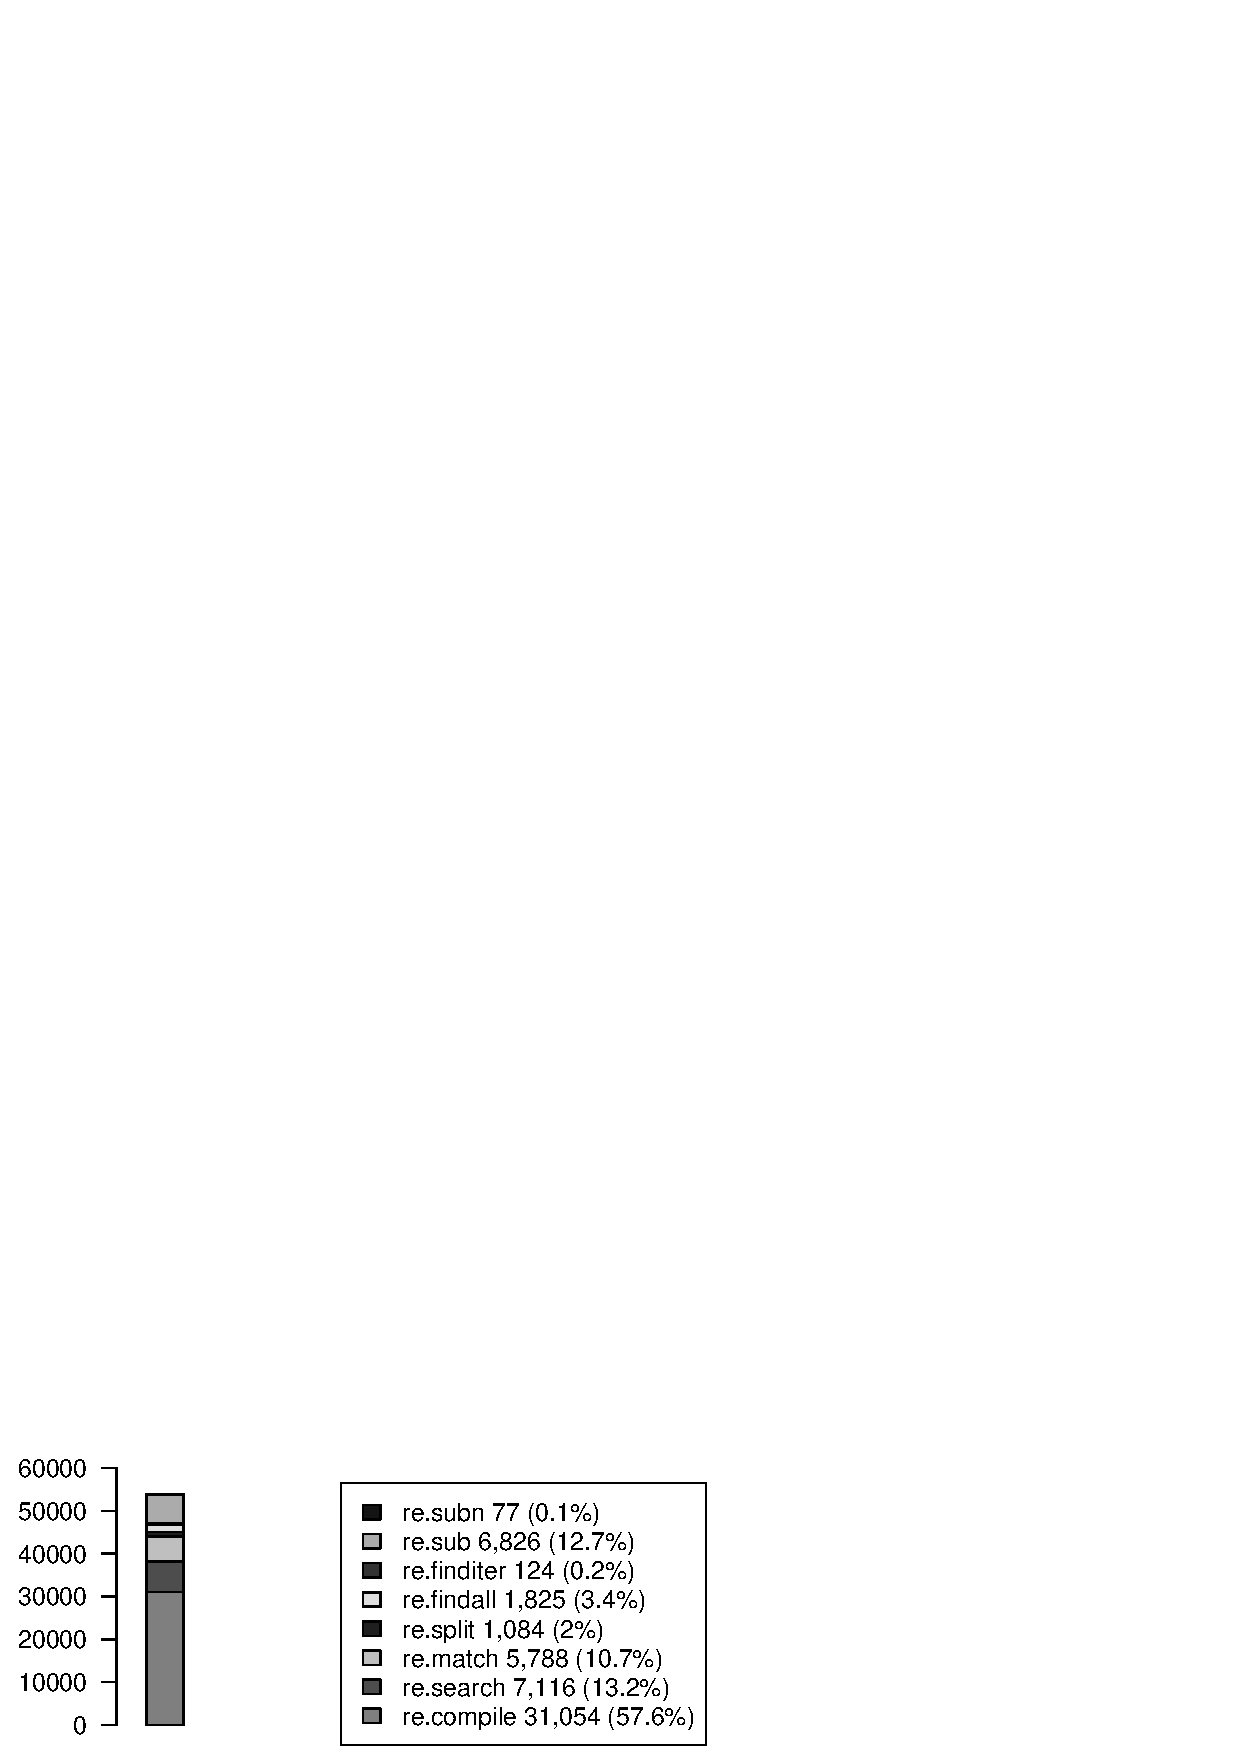
\includegraphics[scale=0.6]{nontex/illustrations/partFunctions.pdf}
%   \label{fig:partFunctions}
% \end{figure}
% \begin{figure}[ht]
%   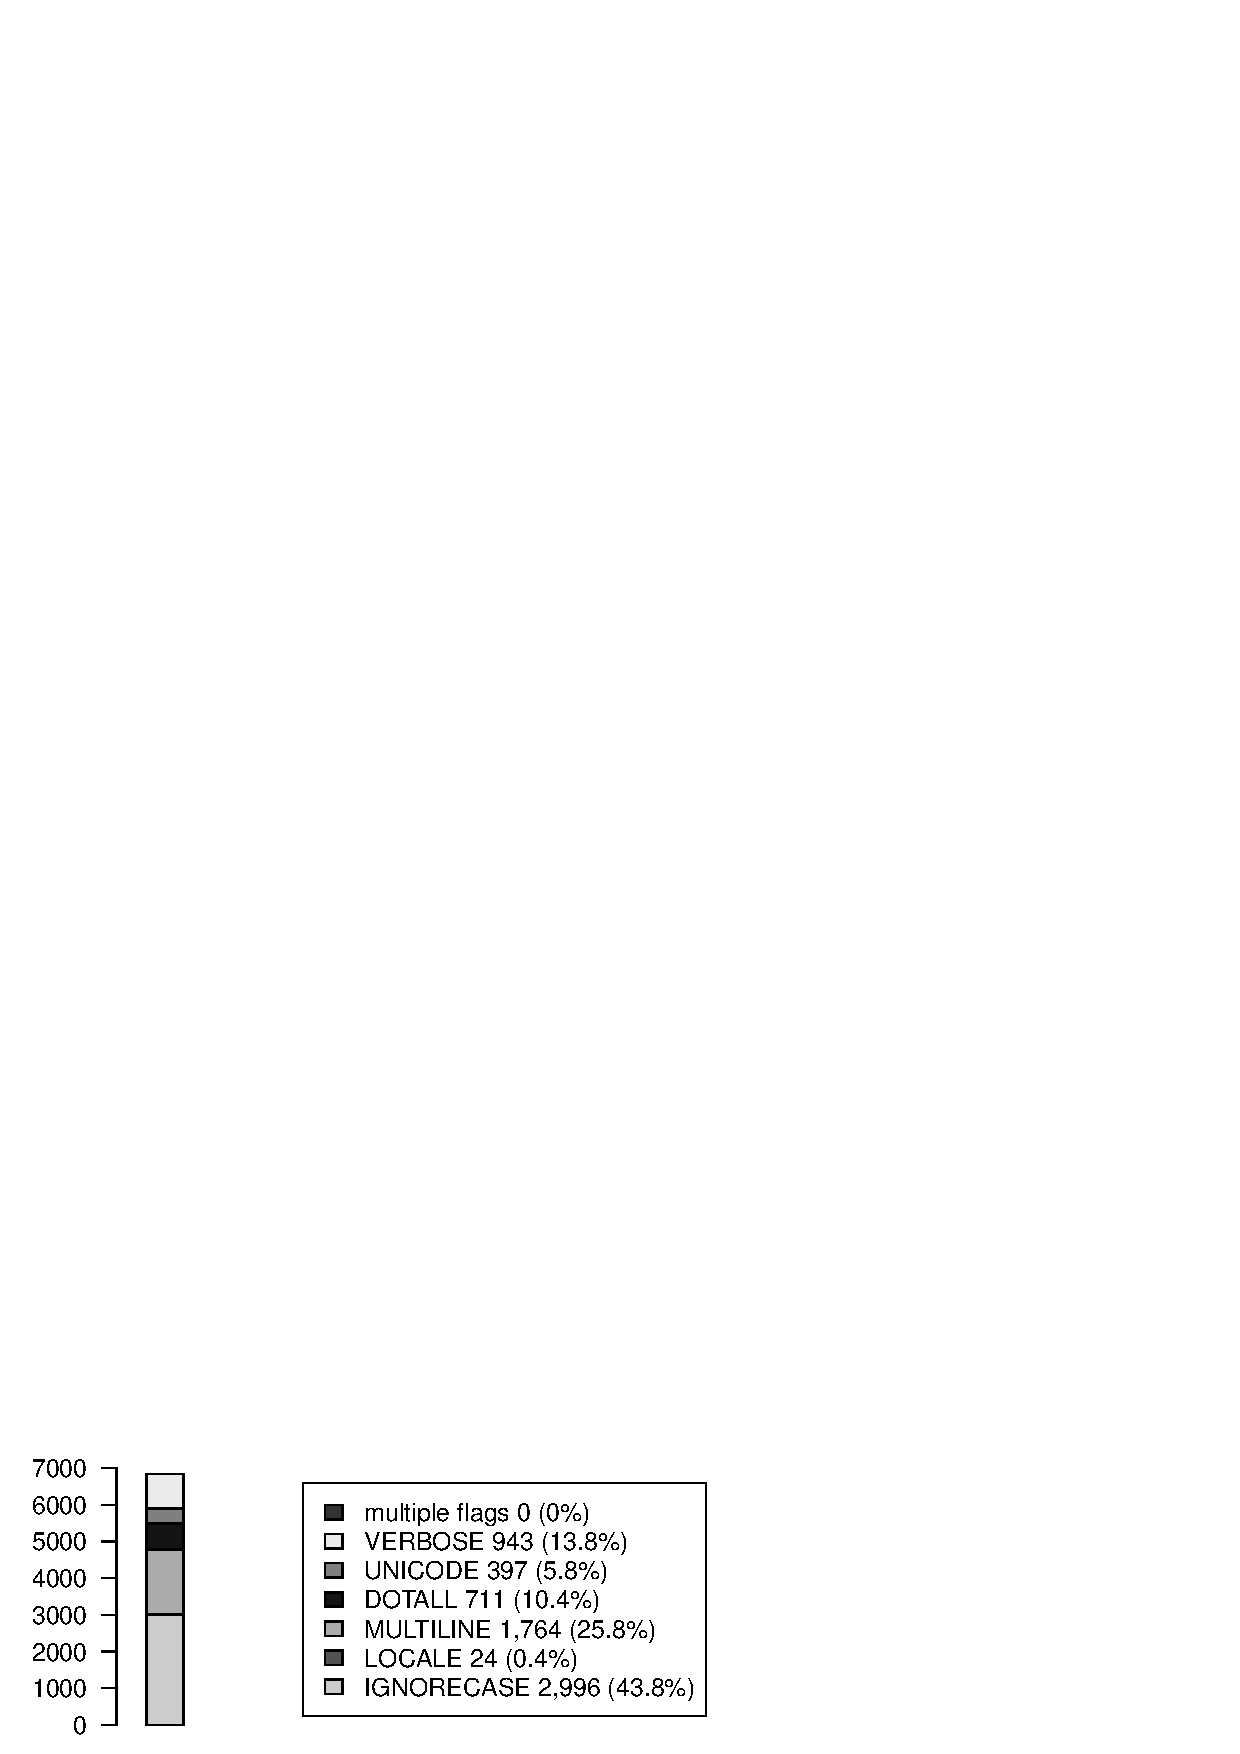
\includegraphics[scale=0.6]{nontex/illustrations/partFlags.pdf}
%   \label{fig:partFlags}
% \end{figure}
% \end{frame}
% \note[itemize]{
%     \item average utilizations per project was 32 and the maximum was 1,427
%     \item each project had an average of 11 files containing any utilization, but med was 6, so there is a skew bc of a few projects with so many
%     \item each of these files had an average of 2 utilizations (med 1)
%     \item avg 2 util. per file
%     \item max 207 util. per file
%     \item max 541 files w/utilizations, med was 2, Q3 was 6...this got skewed
%     \item
% }
%
%% %------------------------------------------------

%recall bias, bad sample of programs, or difference between ephemeral and persistent regexes

\begin{frame}
\frametitle{Notable observations: Features}

\begin{block}{}
\begin{itemize}
	\item {\em Regexes are} (sort of) {\em everywhere} (42\% of projects, 32 utilizations per project)
	\item Current regex research tools cover the most common features
\end{itemize}
\end{block}

\onslide<2->
but....

\onslide<3->
\begin{block}{}
What are the regexes doing?
\end{block}


\end{frame}
